\chapter{Память в виде структурированных хранилищ}\label{ch:ch6}


\newcommand{\up}{\textcolor{green}{$\uparrow$}}
\newcommand{\down}{\textcolor{red}{$\downarrow$}}

\section{Таблица обыкновенная}\label{sec:ch6/sect1}

Графы знаний (KGs) на практике нередко страдают от проблемы неполноты, что существенно снижает их потенциал. Для устранения этой проблемы были разработаны методы завершения графов знаний (KGC). Однако традиционные подходы в этой области отличаются высокой вычислительной сложностью, что делает их неприменимыми для обработки крупномасштабных графов знаний, поскольку они требуют обучения плотных векторных представлений узлов и расчета попарных расстояний.

Генеративные языковые модели на основе трансформеров, такие как T5 и более новая KGT5, представляют собой многообещающую альтернативу, поскольку они способны предсказывать конечные узлы напрямую. В данном исследовании мы предлагаем улучшить методы KGC, основанные на языковых моделях, за счет включения информации о соседних узлах в качестве дополнительного входного параметра.

Результаты наших экспериментов показывают, что предложенный подход превосходит как KGT5, так и традиционные методы KGC на индуктивных и трандуктивных подмножествах Wikidata. Более того, мы детально анализируем влияние информации о соседях на точность предсказаний модели и подтверждаем ее ключевую роль. Наконец, мы указываем направления для значительного улучшения KGC за счет более эффективного выбора соседств.

\section{Introduction}


Графы знаний (KG) представляют собой структурированные данные в виде направленного графа, где узлы обозначают сущности, а рёбра указывают на отношения между ними. Эти сущности могут быть как физическими объектами, так и абстрактными концепциями. Основой каждого графа знаний является набор триплетов, связывающих две сущности через конкретное отношение. Такие триплеты записываются в формате (головная сущность, отношение, конечная сущность) или (h, r, t). Благодаря быстрому развитию этой области графы знаний стали важным инструментом для задач интеллектуального анализа данных, поиска информации, ответов на вопросы и рекомендаций. Тем не менее, многие реальные графы знаний остаются неполными, что ограничивает их возможности. Для устранения этих пробелов алгоритмы дополнения графов знаний (KGC) направлены на предсказание и добавление отсутствующих связей.


\begin{figure}
  \centering
    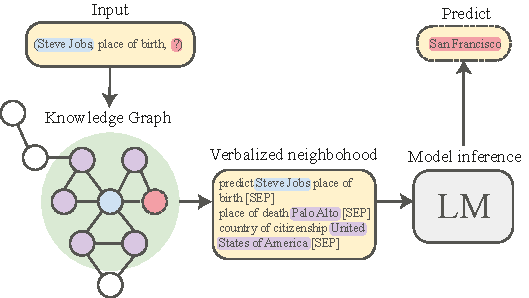
\includegraphics[width=\linewidth]{images/part6/kglm.pdf}
  \caption{\textbf{Процесс дополнения графа.} Из графа знаний (KG) извлекается окружение головного узла триплета, преобразованное в текстовый формат. Языковая модель использует эти текстовые данные для предсказаний, которые могут быть применены в задачах ответа на вопросы или дополнения графа.}
  \label{fig:overall_pipeline}
  \vskip -0.2in
\end{figure}

\section{Векторные представления для графов знаний (KGE)}

Для предсказания связей в KG часто используются векторные представления графов знаний (KGE), которые отражают структурные и семантические особенности узлов, отношений и их контекста. Эти встраивания позволяют функции расстояния различать истинные и ложные триплеты. Однако метод имеет свои ограничения. Потребность в создании уникальных встраиваний для каждого узла и отношения приводит к линейному увеличению размера модели и времени обработки по мере роста графа. Более того, любое обновление KG требует полного переобучения модели, вместо добавления новых встраиваний для изменённых элементов.

\section{Применение языковых моделей в KGC}

Использование языковых моделей (LM) для задач KGC открывает новые перспективы~\cite{pan2023unifying}. Предобученные модели, такие как BERT~\cite{devlin-etal-2019-bert}, GPT-3~\cite{gpt3}, PaLM~\cite{chowdhery2022palm} и LLaMA~\cite{touvron2023llama}, показали выдающиеся результаты в задачах обработки естественного языка (NLP). Эти успехи привели к разработке подходов KGC на базе LM, таких как KG-BERT~\cite{yao2019kgbert}, BERTRL~\cite{zha2022bertrl}, KGT5~\cite{kgt5} и GenKGC~\cite{xie2022discrimination}.

Эти методы рассматривают триплеты KG как текстовые последовательности. В отличие от методов, основанных на расстояниях, которые акцентируют внимание на структуре, языковые модели лучше улавливают семантику сущностей и отношений. Это позволяет LM-методам работать с ранее неизвестными сущностями и делать выводы о новых фактах, используя текстовые представления триплетов. Например, модель KGT5 преобразует задачу предсказания связей в KG в задачу последовательного преобразования. Обучаясь на предсказании конечного узла по текстовым данным триплета, KGT5 демонстрирует конкурентоспособные результаты, предоставляя простой и масштабируемый подход для задач KGC и ответа на вопросы.

Большинство методов на базе LM, таких как KG-BERT, BERTRL, KGT5 и GenKGC, основываются исключительно на знаниях, содержащихся в параметрах языковой модели. Однако граф знаний предоставляет дополнительную информацию, которую можно использовать. Мы предлагаем метод, объединяющий внутренние знания языковых моделей с внешними данными из KG. Для задачи предсказания связей ($h$, $r$, $?$) наш подход использует окружение узла $h$, то есть связанные с ним узлы и отношения. Окружение узла нередко содержит полезные подсказки. Например, для триплета (Стив Джобс, место рождения, ?) информация об «окрестности», включающая такие сущности, как «Пало-Альто» и «США», помогает точнее представить головной узел.

Хотя некоторые исследования уже рассматривали включение окружения в алгоритмы KGC~\cite{chen2020hitter}, наш подход отличается использованием преимуществ генеративных языковых моделей в сравнении с KGE. Основные преимущества: (1) масштабируемость и компактность модели, (2) возможность обобщать данные на новые сущности, что делает метод подходящим как для трандуктивных, так и для индуктивных графов знаний, (3) отсутствие необходимости ранжировать всех возможных кандидатов для триплетов благодаря прямой генерации конечного узла. Также параллельное исследование авторов KGT5, известное как KGT5-context~\cite{kochsiek2023friendly}, подтверждает эффективность включения окружения узлов в генеративные языковые модели для задач KGC.


Наш вклад

1. Мы разработали новый метод генеративного дополнения графов, который сочетает языковые модели и информацию о соседних элементах графа.  
2. Экспериментально показано, что добавление графовой информации в генеративные языковые модели значительно улучшает результаты предсказания связей как в трансдуктивных, так и в индуктивных задачах. Кроме того, предложенный метод установил новые передовые результаты на индуктивном наборе данных ILPC.  
3. Мы провели анализ и оценку влияния добавления информации о соседях на точность и эффективность работы моделей.  


\section{Методы}

Граф знаний (KG) формально представляется в виде \(\mathcal{G} = (\mathcal{T}, \mathcal{E}, \mathcal{R})\), где \(\mathcal{E}\) обозначает множество сущностей, \(\mathcal{R}\) — множество отношений, а \(\mathcal{T}\) — множество триплетов, \(\mathcal{T} \in \mathcal{E} \times \mathcal{R} \times \mathcal{E}\). Задача дополнения графа знаний (KGC) заключается в следующем: для триплета \(\mathcal{T}_{i} = (h, r, t)\), где \(h, t \in \mathcal{E}\) и \(r \in \mathcal{R}\), необходимо ответить на запросы вида \((h, r, ?)\) и \((?, r, t)\), исключив данный триплет из графа \(\mathcal{G}\).

Существуют различные подходы к решению задач KGC, которые зависят от типа графа. В трансдуктивной постановке модель обучается на графе \(\mathcal{G}_{train} = (\mathcal{T}_{train}, \mathcal{E}, \mathcal{R})\) и тестируется на графе \(\mathcal{G}_{inference} = (\mathcal{T}_{inference}, \mathcal{E}, \mathcal{R})\), где множества сущностей и отношений остаются одинаковыми. В индуктивной задаче модель обучается на графе \(\mathcal{G}_{train} = (\mathcal{T}_{train}, \mathcal{R}, \mathcal{E}_{train})\) и тестируется на графе \(\mathcal{G}_{inference} = (\mathcal{T}_{inference}, \mathcal{R}, \mathcal{E}_{inference})\), что требует обработки ранее невиданных сущностей.

Наш подход основан на методике KGT5~\cite{kgt5}, где для решения задачи KGC применяется трансформер с архитектурой "кодировщик-декодировщик", основанный на T5~\cite{raffel2020t5}. Задача предсказания связей заключается в поиске недостающего элемента триплетов \((entity_1, relation, entity_2)\) через решение запросов \((entity_1, relation, ?)\) и \((entity_2, relation^{-1}, ?)\).

Для подготовки входных данных запросы преобразуются в текстовый формат. Помимо вериализации запросов, как предложено в KGT5, мы добавили информацию о соседних элементах графа для каждого триплета. Эта информация включает узлы и отношения, соединённые с головным узлом триплета (соседи первого уровня). Если количество соседей превышает допустимую длину контекста модели, их отбирают на основе семантического сходства отношений, оставляя только те, которые помещаются в заданный лимит длины последовательности.

Для оценки предложенного метода мы использовали общедоступные трансдуктивные и индуктивные графы знаний. Были протестированы Wikidata5M~\cite{wang2021kepler} — один из крупнейших трансдуктивных наборов данных, а также крупные и малые версии ILPC~\cite{ilpc} — крупнейшего полностью индуктивного набора данных. Графы из ILPC характеризуются большой размерностью и разреженностью, что создаёт серьёзные трудности для существующих методов, таких как GNN~\cite{ilpc}. Эти особенности приводят к относительно низким метрикам точности, при этом пока ни один из подходов не смог превзойти базовый уровень, предложенный в статье ILPC. Оба набора данных представляют собой подмножества реального графа знаний Wikidata.

Чтобы проверить нашу гипотезу о том, что информация о соседях улучшает представление узлов графа, мы сравнили модели, обученные с учётом соседей и без них. Кроме того, в отличие от KGT5, мы протестировали различные настройки, включая дообучение предварительно обученных моделей и обучение с нуля, предполагая, что предварительное обучение на языковых данных может быть полезным для реальных графов знаний, таких как Wikidata.

В наших экспериментах использовалась модель T5-small с 60M параметров. Мы оценивали модели как с предварительно обученными весами, так и с случайной инициализацией, чтобы изучить влияние предобучения. Токенизатор был дополнен специальными токенами "[SEP]" для разделения запросов и информации о соседях. Обучение проводилось с использованием оптимизатора AdamW~\cite{loshchilov2018adamw}, скорости обучения \(1e{-5}\), дропаутом 10\% и размером батча 320. Для Wikidata5M обучение включало 5M шагов, а для остальных наборов данных — 2M шагов. Для распределённого обучения на нескольких GPU применялась платформа Horovod~\cite{horovod}. В случаях, когда размер батча превышал доступную память GPU, использовалась стратегия накопления градиентов.

Кроме того, мы протестировали OpenAI \texttt{gpt-3.5-turbo}\footnote{\texttt{gpt-3.5-turbo-0613}: \url{https://platform.openai.com/docs/models/gpt-3-5}} для задач предсказания связей без обучения, чтобы оценить, как информация о соседях влияет на крупные языковые модели. Исходный код всех экспериментов доступен в репозитории\footnote{\url{https://github.com/screemix/kgc-t5-with-neighbors}}.  
\label{sec:training}

Модель KGT5 создает распределение вероятностей для каждого токена из словаря на всех этапах декодирования. Это распределение корректируется штрафами за расхождения с истинным распределением, то есть за несоответствие между целевым токеном в позиции $i$ и предсказанным токеном на шаге $i$, с использованием функции потерь на основе перекрестной энтропии (CE loss).

Данный метод значительно отличается от подходов, основанных на измерении расстояния, поскольку он не требует создания негативных примеров для их отдаления от правильного предсказания в каждом обучающем запросе. Это делает процесс обучения независимым от размера графа знаний (KG).

Для получения предсказаний мы сначала преобразуем запрос (head,relation,?)(head,relation,?) в вербализованный вид и вводим его в генеративную модель, которая генерирует последовательность, представляющую вербализованный идентификатор целевой сущности. Для выполнения вывода мы применили две стратегии.

Первая стратегия заключается в выборке kk наиболее вероятных последовательностей из декодера. Следуя настройкам KGT5~\cite{kgt5}, мы выбрали размер выборки, равный 50, и применили этот подход к трандуктивному набору данных Wikidata5M. Вторая стратегия заключается в поиске сущностей в графе знаний, наиболее близких к сгенерированной сущности. Этот подход был применен к индуктивным наборам данных ILPC, где модели должны генерировать сущности, ранее не встречавшиеся в обучении.

\begin{table*}[htp] \caption{Учет информации о соседях стабильно повышает качество выполнения задачи предсказания связей. В таблице представлены метрики Hits@k для тестовых наборов данных Wikidata5M, ILPC-small и ILPC-large. Стрелки (↑↑, ↓↓) демонстрируют влияние информации о соседях на производительность языковых моделей. Учет соседей позволяет достичь наилучших результатов с учетом числа параметров модели.}
\vskip -0.1in
\label{tab:triplet-results}
\centering
\resizebox{\textwidth}{!}{
\begin{tabular}{@{}llllllllllll@{}}
\toprule
\multirow{2}{*}{Model} & \multicolumn{3}{c}{Wikidata5M} & \multicolumn{3}{c}{ILPC-small} & \multicolumn{3}{c}{ILPC-large}  &  \\
\cmidrule(lr){2-4}\cmidrule(lr){5-7}\cmidrule(lr){8-10}
& H@1 & H@3 & H@10 & H@1 & H@3 & H@10 & H@1 & H@3 & H@10 & \#params \\
\midrule
KGT5~\cite{kgt5} & 0.267 & 0.318 & 0.365 & - & - & - & - & - & - & 60M\\
TransE~\cite{transe} & 0.170 & 0.311 & 0.392 & - & - & - & - & - & - & 2,400M \\
ComplEx~\cite{complex} & 0.255 & - & 0.398 & - & - & - & - & - & - & 614M \\
KEPLER~\cite{wang2021kepler} & 0.173 & 0.224 & 0.277 & - & - & - & - & - & - & 125M \\
SimKGC~\cite{wang2022simkgc} & 0.313 & 0.376 & 0.441 & - & - & - & - & - & - & 220M \\
IndNodePiece~\cite{ilpc} & - & - & - & 0.007 & 0.022 & 0.092 & 0.037 & 0.054 & 0.125 & 15.5K \\
IndNodePieceGNN~\cite{ilpc} & - & - & - & 0.076 & 0.140 & 0.251 & 0.032 & 0.073 & 0.146 & 24K\\

\midrule
T5-small not pre-trained & 0.240 & 0.286 & 0.323 & - & - & - & - & - & - & 60M\\
T5-small not pre-trained + neighbors & 0.327\up & 0.363\up & 0.386\up & - & - & - & - & - & - & 60M\\
T5-small pre-trained & 0.205 & 0.248 & 0.282 & 0.073 & 0.117 & 0.177 & 0.112 & 0.137 & 0.194 & 60M\\
T5-small pre-trained + neighbors & 0.306\up & 0.342\up & 0.361\up & 0.076\up & 0.137\up & 0.209\up & 0.114\up & 0.139\up & 0.200\up & 60M\\
T5-base pre-trained & - & - & - & 0.073 & 0.130 & 0.199 & 0.110 & 0.136	& 0.198 & 220M\\
T5-base pre-trained + neighbors & - & - & - & 0.082\up & 0.142\up & 0.216\up & 0.116\up & 0.141\up & 0.215\up & 220M \\

\bottomrule
\end{tabular}
}
\vskip -0.1in
\end{table*}

\section{Results}


Наш метод основан на предположении, что добавление информации о соседях в контекст, предоставляемый языковой модели, способно улучшить предсказание связей при использовании генеративных языковых моделей. Результаты, представленные в таблицах~\ref{tab:ablation} и \ref{tab:chatgpt}, показывают, как наш подход работает на наборах данных Wikidata5M и ILPC при различных условиях. Среди них обучение модели T5 с использованием информации о соседях и без нее, применение предварительно обученной модели или обучение модели с нуля, а также zero-shot оценка с \texttt{gpt-3.5-turbo}.

Результаты подтверждают, что учет информации о соседях способствует улучшению качества предсказания связей в генеративных моделях как в трансдуктивной, так и в индуктивной средах. В частности, наш подход показал SOTA-результаты на наборе данных ILPC, а на Wikidata5M достиг лучших показателей среди генеративных моделей предсказания связей. Эти показатели сопоставимы с результатами SOTA-методов, основанных на графах и языковых моделях, которые используют значительно больше параметров. Относительно низкие значения оценок на наборе данных ILPC можно объяснить его полностью индуктивной природой и большей разреженностью по сравнению с Wikidata5M. Заметим, что на текущий момент нет общедоступных решений, превышающих базовый результат, предложенный авторами ILPC. Наше решение не только превосходит существующую базовую линию, но также отличается простотой и более высокой интерпретируемостью по сравнению с методами на основе GNN.

Эксперименты с предварительно обученными моделями показали, что предварительное обучение ускоряет процесс сходимости, но снижает качество модели на несколько пунктов по сравнению с обучением с нуля.

Кроме того, мы подтвердили, что информация о соседях повышает производительность различных генеративных моделей. Это справедливо как для открытых моделей, таких как T5, так и для проприетарных моделей, например, GPT от OpenAI, предоставляемых в формате «модель как услуга». У каждого типа моделей есть свои сильные и слабые стороны. Например, GPT от OpenAI являются моделями «черного ящика», которые не подлежат модификации или интерпретации, что ограничивает их применение для специализированных или проприетарных графов знаний, содержащих конфиденциальные данные. Несмотря на больший размер и высокую стоимость \texttt{gpt-3.5-turbo} от OpenAI по сравнению с компактной и прозрачной моделью T5, наш метод показывает улучшение производительности обеих моделей.

\begin{table} \caption{Эффект использования информации о соседях на предсказание связей в режиме zero-shot с OpenAI \texttt{gpt-3.5-turbo-0613}. *Результаты на ILPC-Large рассчитаны на основе 5000 случайных выборок из тестового набора. }
\vskip -0.1in
\label{tab:chatgpt}
\centering
\resizebox{0.48\textwidth}{!}{
\begin{tabular}{@{}lllllll@{}}
\toprule
\multirow{2}{*}{Dataset} & \multicolumn{2}{c}{GPT} & \multicolumn{2}{c}{GPT+NEIGH}  \\
\cmidrule(lr){2-3}\cmidrule(lr){4-5}
& H@1 & H@3 & H@1 & H@3 \\
\midrule
Wikidata5M & 0.098 & 0.131 & 0.113\up & 0.157\up \\
ILPC-small & 0.079 & 0.107 & 0.084\up & 0.118\up  \\
ILPC-large* & 0.103 & 0.134 & 0.114\up & 0.150\up  \\
\end{tabular}
}
\vskip -0.2in
\end{table}

Чтобы разобраться, как предложенные модели используют соседние триплеты, мы провели сравнение предсказаний моделей, обученных с использованием графовой информации во входных данных, и без нее. Один из случаев, когда соседние данные оказываются полезными для предсказания связей, возникает тогда, когда целевая сущность косвенно присутствует во входных данных модели. Из-за фильтрации соседств целевой триплет исключается из входных данных, но целевая сущность все же может быть представлена через другие отношения, как подстрока в другой сущности или даже в контексте самой задачи (см. Таблицу~\ref{tab:target_inclusion}).

Несмотря на то что хвостовая сущность появляется во входных данных только в небольшой части тестового набора, модель с использованием соседств эффективно использует такие косвенные подсказки. Во всех протестированных сценариях она показывает результаты лучше, чем базовая модель T5. Высокий уровень решения — более 80% в случаях с подсказками, связанными с целевой сущностью, — подчеркивает важность тщательно отобранных соседств.

\begin{figure}[h]
  \centering
    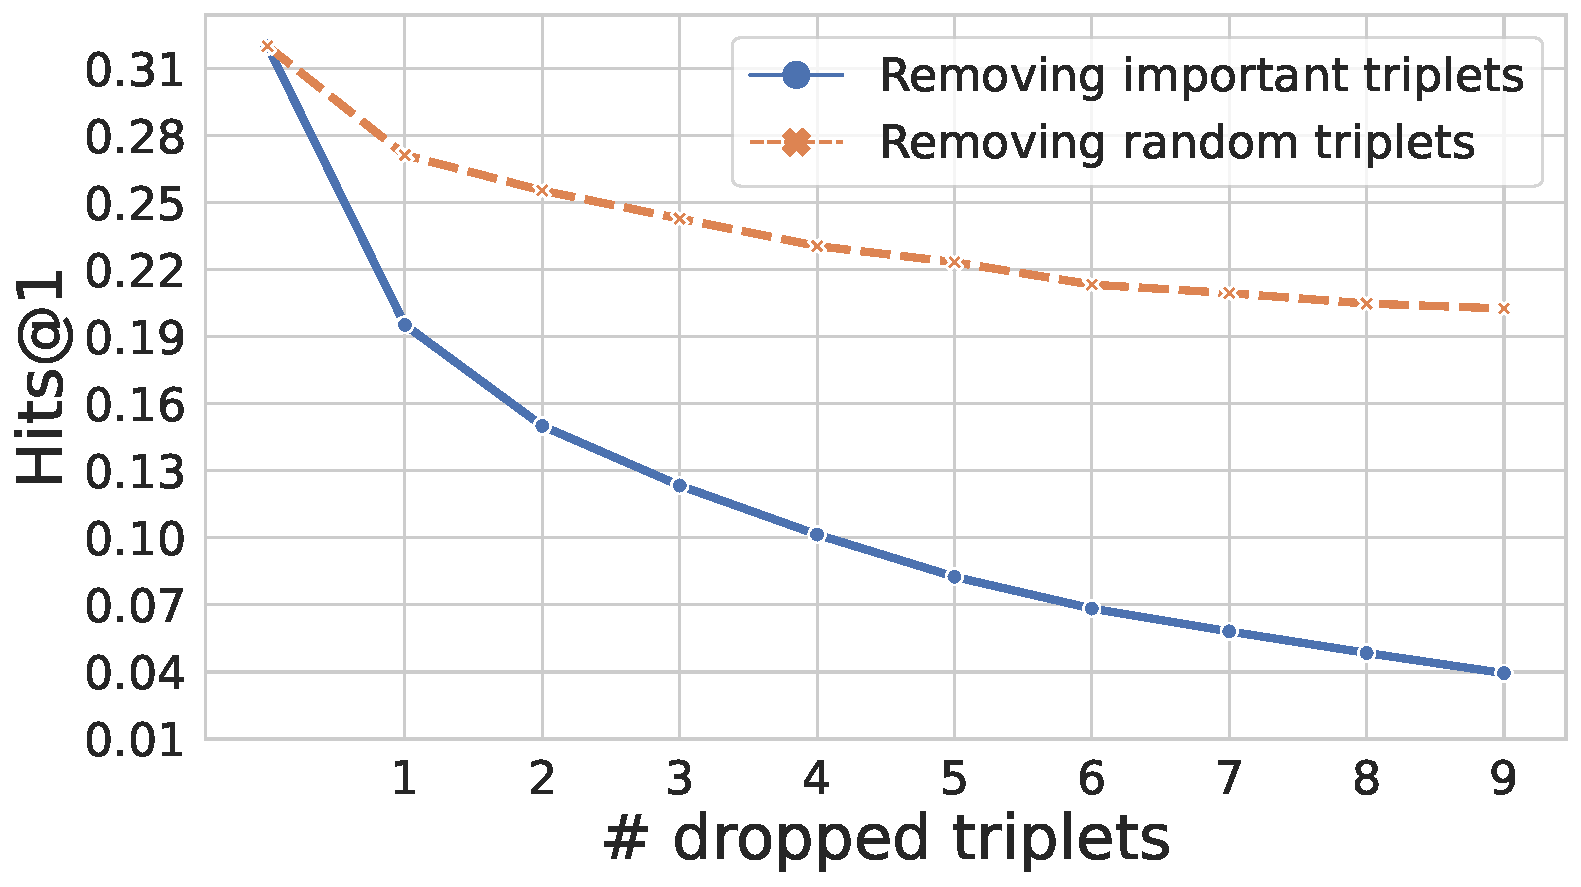
\includegraphics[width=\linewidth]{images/part6/output.pdf}
  \caption{\textbf{Роль графового соседства в производительности модели.} На графике показано, как удаление соседних триплетов влияет на качество предсказания связей с использованием датасета Wikidata5M и модели T5-small без предварительного обучения. Сплошная синяя линия отражает удаление наиболее значимых триплетов, пунктирная красная линия — случайное удаление.}
  \label{fig:interptretation}
  \vskip -0.1in
\end{figure}

Для изучения значимости соседств мы проанализировали важность триплетов, отсортировав их в зависимости от их влияния на вероятность предсказания целевого узла. Как видно из Рисунка~\ref{fig:interptretation}, производительность модели заметно снижается при удалении ключевых триплетов из контекста. Это указывает на то, что включение значимых триплетов на этапах предобработки или обучения может значительно улучшить результаты. Кроме того, анализ карт внимания модели, обученной на Wikidata5M, показал, что она сосредотачивает внимание на релевантных соседних триплетах.

Результаты анализа подтверждают, что добавление графового контекста существенно улучшает предсказание связей. Одной из стратегий повышения производительности является расширение размера соседства за счет включения соседей через k шагов. Однако квадратичная сложность механизмов внимания в трансформерах и ограничение на размер входных данных затрудняют обработку экспоненциально растущих соседств.

Использование более эффективных архитектур трансформеров, таких как модели T5 с размером входных данных до 32k токенов \cite{guo-etal-2022-longt5} и 64k токенов \cite{ainslie2023colt5}, или рекуррентных подходов, например, \cite{rmt_2022,hutchins2022blockrecurrent}, позволяет справляться с большими соседствами. Еще одним подходом может быть выбор подграфов, включающих более удаленную, но релевантную информацию, например, через случайные блуждания или сложные методы \cite{das2018minerva}.

\begin{table}%[h]
  \caption{Повышение точности предсказаний связей для T5-small на тестовом наборе Wikidata с использованием релевантных соседей. Таблица отражает точность совпадений в зависимости от косвенного присутствия целевой сущности во входных данных модели.}
  \label{tab:target_inclusion}
  \begin{tabular}{lccr}
    \toprule
    Target position &  T5 & T5 + Neighbors & frequency\\
    \midrule
    In task         & 0.93 & 0.94 \up & 5 \%  \\
    In neighborhood & 0.34 & 0.82 \up & 8 \% \\
    Not in input    & 0.18 & 0.24 \up & 87 \% \\
    Total           & 0.23 & 0.32 \up & 100 \% \\
  \bottomrule
\end{tabular}
\vskip -0.1in
\end{table}

Выводы и дальнейшие исследования

В ходе работы было установлено, что использование данных о соседних узлах графа знаний (KG) в контексте генеративной модели способствует повышению качества выполнения задач предсказания связей. Мы обучили модель T5-small на трандуктивных данных (Wikidata5M) и индуктивных наборах (ILPC) с различными параметрами и доказали, что одновременное представление узла и его соседей обеспечивает более точное моделирование. Представленный подход значительно превосходит существующие аналоги на крупнейших реальных наборах для дополнения графов знаний (KGC), обеспечивая это при меньшем или равном количестве параметров. Также установлено, что производительность \texttt{gpt-3.5-turbo} от OpenAI улучшается при использовании данных о соседях, даже без предварительной настройки. Помимо улучшений качества, исследование выявило важность импутации соседей. В будущем следует сосредоточить усилия на оптимизации выбора значимых триплетов и расширении контекста моделей. Другие перспективы включают анализ влияния размера моделей, изучение методов импутации на других областях и усовершенствование алгоритмов выбора соседей.
Ограничения

Работа ограничена использованием моделей относительно небольшого размера, таких как T5, что оставляет открытым вопрос о преимуществах крупных моделей для задач KGC. Кроме того, каждая модель применялась только к одному графу знаний, что не позволяет учесть особенности сложных графов, охватывающих несколько наборов данных. Еще одним ограничением является общий характер языковых моделей, которые могут быть менее эффективны в специализированных областях, например, биологии или медицине. Оптимальность выбранных соседей не гарантируется, что требует дальнейших исследований для улучшения охвата графов и отбора наиболее релевантных узлов. Кроме того, используемые запросы для оценки GPT-моделей могут быть не полностью оптимизированы, поскольку отсутствие точных данных о тренировках модели снижает вероятность достижения максимальных показателей.

\section{Построение графов знаний из текстов}

Предложенный метод ориентирован на расширение графов знаний, таких как Wikidata, за счет извлечения триплетов из текстов с помощью крупных языковых моделей (LLMs). Методика включает два этапа: определение кандидатов на сущности и их последующее уточнение с привязкой к каноническим элементам и связям графа. Проверка точности осуществляется с использованием ограничений отношений в Wikidata. Сравнение с моделью, обученной на синтетическом наборе, показало, что предложенный подход обеспечивает более высокую точность на естественных данных. Результаты подтверждают, что извлечение триплетов с применением LLM и механизмов проверки является эффективным инструментом для практического использования.

\section{Introduction}

\begin{figure*}[t]
  \centering
    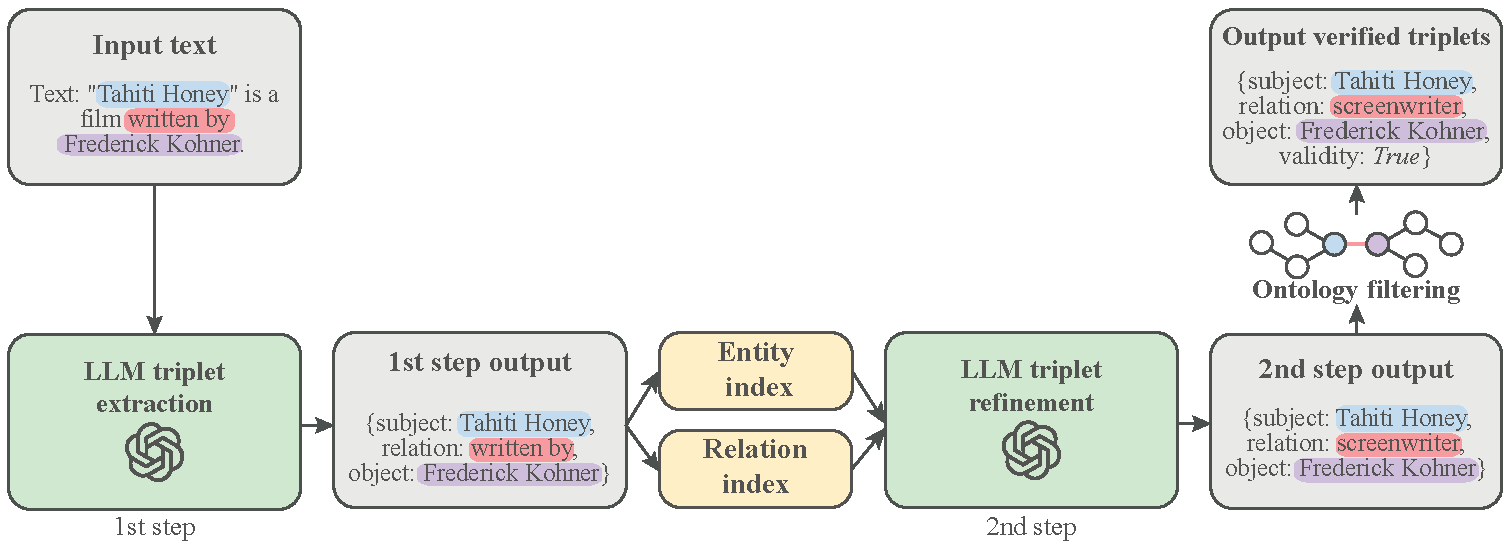
\includegraphics[width=0.9\textwidth]{images/part6/pipeline.pdf}
  \caption{\textbf{Методика расширения графа знаний (KG).} На первом этапе с помощью LLM и подхода на основе промптов из текста извлекаются триплеты, формирующие JSON-список, который может содержать неточности в названиях сущностей и отношений. Затем канонические названия сущностей и отношений извлекаются и включаются в промпт LLM для уточнения триплетов. На завершающем этапе уточненные триплеты проверяются на соответствие онтологии KG для обеспечения их согласованности. }
  \label{fig:full_pipeline}
  \vskip -0.2in
\end{figure*}

Современные знания в основном представлены в неструктурированном виде, например, в книгах, статьях, новостях, блогах и социальных сетях. Графы знаний (KG) играют ключевую роль в преобразовании этих данных в структурированный формат, делая их более доступными и применимыми в различных сферах. WikiData~\cite{vrande2012wikidata} — один из крупнейших открытых графов знаний, содержащий более 1,54 миллиарда элементов, поддерживаемый международным сообществом. Однако поддержание его актуальности требует значительных усилий. Автоматизация пополнения KG на основе извлеченной из текста информации может стать эффективным решением этой задачи, помогая ресурсам оставаться актуальными и легко обновляемыми.

Графы знаний представляют собой направленные многореляционные графы, где узлы соответствуют сущностям, а ребра описывают их взаимосвязи. Эти структуры описываются с помощью триплетов вида (основная сущность, отношение, зависимая сущность) или (h, r, t), создавая организованное представление фактов о реальных и абстрактных объектах.

Извлечение знаний или триплетов — важный шаг в автоматическом создании масштабных KG. Оно включает обнаружение сущностей и их отношений в неструктурированных текстах. Процесс, как правило, включает три этапа: 1) обнаружение сущностей, 2) разрешение кореференций и 3) извлечение отношений. Ошибки, возникающие на любом из этапов, например, при обнаружении сущностей, могут отрицательно сказаться на результатах.

Современные методы направлены на объединенное извлечение сущностей и отношений, рассматривая задачу как проблему последовательного обучения с использованием генеративных языковых моделей (LM) \cite{melnyk2021grapher}. Такой подход минимизирует распространение ошибок и повышает производительность без необходимости в дополнительной разметке данных.

Однако обучение специализированных LM для конкретных KG сопряжено с проблемами, такими как требование больших размеченных данных и частое переобучение для новых версий KG или других областей. Более того, такие модели часто ограничены только теми сущностями и отношениями, которые были доступны в прошлых версиях KG или других онтологиях.

Крупные языковые модели (LLM), такие как ChatGPT и GPT-4, благодаря своим универсальным возможностям анализа и генерации текста, становятся перспективными для построения KG. В то время как традиционные методы зависят от тонкой настройки последовательных моделей, недавние исследования показывают, что LLM могут извлекать триплеты через обучение на контексте (ICL)~\cite{brown2020language} и следование инструкциям~\cite{ouyang2022training}. Эти методы не требуют дообучения, так как основаны на использовании специально разработанных промптов и механизма сопоставления сущностей и отношений с каноническими именами KG.

В данной работе мы исследуем применение LLM для извлечения знаний и расширения KG, ориентируясь на Wikidata. Мы представляем новую трехэтапную методику, включающую: 1) генерацию начальных кандидатов для сущностей и отношений с помощью LLM; 2) уточнение триплетов через сопоставление с каноническими именами из KG; 3) валидацию уточненных триплетов с использованием онтологии KG для обеспечения их точности. Мы также проводим оценку предложенного подхода и модели, обученной на наборе данных SynthIE, для анализа их эффективности на реальных данных.

\section{Methods}
\begin{figure*}[t]
  \centering
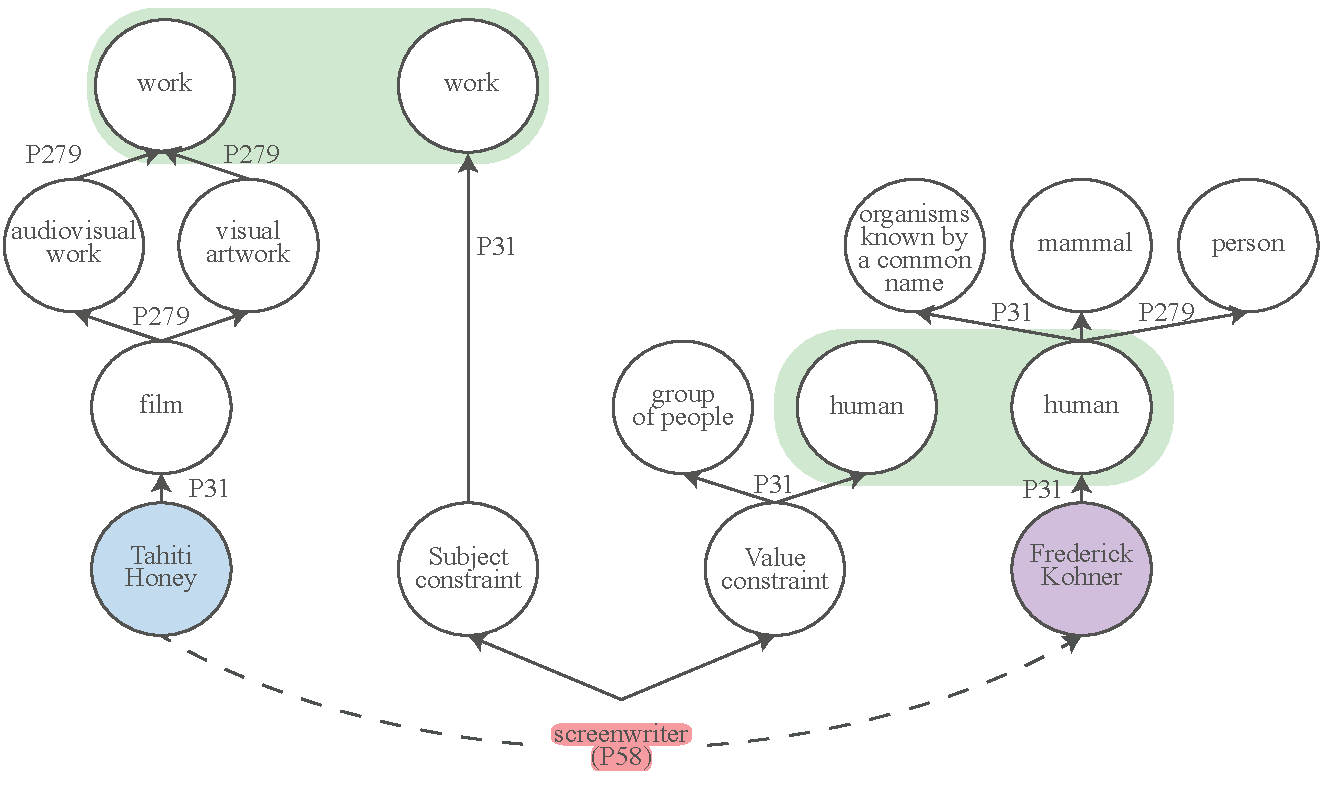
\includegraphics[width=0.7\textwidth]{images/part6/ontology-verification.pdf}
Триплеты, сформированные в рамках предложенного конвейера, проходят проверку на основе онтологии для обеспечения их соответствия структуре онтологии графа знаний (KG). Триплет считается корректным, если типы в иерархии субъекта и объекта пересекаются с типами, указанными в ограничениях для заданного отношения. Для упрощения иллюстрации структура онтологии была сокращена. Сокращения P31 и P279 обозначают отношения \textit{"экземпляр"} и \textit{"подкласс"} соответственно.

\label{fig:ontology}
\vskip -0.2in
\end{figure*}

Для извлечения триплетов из текста мы разработали многоэтапный конвейер (Рисунок~\ref{fig:full_pipeline}). Первый этап (Раздел~\ref{sec:1st_step}) включает извлечение кандидатов на триплеты. Эти кандидаты могут содержать сущности и отношения, которые не соответствуют форматам, принятым в Wikidata KG. На втором этапе (Раздел~\ref{sec:triplet-retrieval}) выполняется уточнение кандидатов за счёт сопоставления их с похожими сущностями и отношениями из KG. На завершающем этапе уточнённые триплеты проходят проверку на соответствие онтологии KG (Раздел~\ref{sec:filtration}), включая проверку ограничений отношений и совместимости типов сущностей. Для реализации первых двух этапов конвейера используется модель OpenAI \texttt{gpt-3.5-turbo}, которая работает с учётом заданных примеров и инструкций.
Наборы данных

Создание наборов данных для извлечения триплетов представляет собой сложную и трудоёмкую задачу. Аннотаторам необходимо понимать все сущности и отношения в KG, чтобы корректно интерпретировать факты, содержащиеся в тексте. Для крупных графов знаний, таких как Wikidata, это становится особенно сложной задачей, что ограничивает доступность качественных наборов данных для построения KG. Большинство существующих наборов данных либо фрагментарны, либо содержат шум. Например, популярный набор данных REBEL~\cite{huguet-cabot-navigli-2021-rebel} часто не предоставляет достаточно информации для извлечения сущностей из текста, заменяя их местоимениями. Более того, целевые триплеты в REBEL часто бывают неполными или содержат неточности по отношению к исходному тексту~\cite{josifoski2023exploiting}. Подобные проблемы наблюдаются и в других популярных наборах данных~\cite{josifoski2021genie}.

Оценка моделей на наборах данных с удалённым супервизированием, таких как REBEL, обычно приводит к существенным ошибкам в оценке производительности. В связи с этим мы использовали более качественный набор данных SynthIE~\cite{josifoski2023exploiting}. Хотя этот набор данных создан синтетически, его авторы подчёркивают, что крупные языковые модели (LLM) испытывают сложности в решении задач извлечения информации. Эта задача считается асимметричной, так как LLM способны генерировать текст на основе триплетов KG, но не наоборот.
Извлечение кандидатов на триплеты

\label{sec:1st_step}
На первом этапе из входного текста извлекаются кандидаты на триплеты. Мы протестировали модель OpenAI \texttt{gpt-3.5-turbo}\footnote{\texttt{gpt-3.5-turbo-0125}: \url{https://platform.openai.com/docs/models/gpt-3-5}} в задаче извлечения триплетов, предоставив контекст с примерами. В подсказке было описано задание и приведено три примера из обучающего набора данных Wiki-cIE Code~\cite{josifoski2023exploiting}.

Например, для текста:
\textit{"Tahiti Honey" is a film written by Frederick Kohnner} would be:
\textit{"Tahiti Honey", "written by", "Frederick Kohner"}.

Однако извлечённые сущности и отношения не всегда нормализованы, то есть могут не соответствовать правилам именования, принятым в исходном KG.
Уточнение кандидатов на триплеты

\label{sec:triplet-retrieval}
Основным ограничением LLM в задачах построения KG является их неспособность надёжно сопоставлять извлечённые имена с каноническими сущностями и отношениями Wikidata. Чтобы устранить эту проблему, мы применили двухэтапную стратегию подсказок. После извлечения триплетов на первом этапе мы использовали FAISS~\cite{faiss} для поиска канонических имён из Wikidata KG, ранжированных по косинусному сходству с извлечёнными сущностями и отношениями.

Индекс был построен с использованием предварительно обученных эмбеддингов Contriever~\cite{contriever}, которые демонстрируют высокую устойчивость и производительность в различных задачах поиска. Среди пяти наиболее подходящих канонических имён, предложенных для каждой сущности и отношения, необходимо выбрать те, которые лучше всего соответствуют контексту текста и триплета.

Например, для вышеупомянутого триплета система предложит пять канонических имён, ранжированных по сходству с извлечённым субъектом, объектом и отношением: \


\textit{"written by": ["lyrics by", "adapted by", "produced by", "screenwriter", "author"]}

\textit{"Tahiti Honey": ["Tahiti Honey", "Honey", 
"Honey Chile", "Celtic Honey", "Tahitipresse"]}

\textit{"Frederick Kohner": ["Frederick Kohner",
"Paul Kohner", "Adolf Kohner", "Susan Kohner", "Henry Rohner"]}

As a result, after choosing the corresponding names that fit the context of the text, the refined triplet is
\textit{"Tahiti Honey", "screenwriter", "Frederick Kohner"}

\subsection{Ontology-based verification}
\label{sec:filtration}
Для повышения достоверности результатов работы пайплайна в условиях возможных галлюцинаций крупных языковых моделей (LLM) нами разработан метод автоматической проверки триплетов, основанный на использовании онтологии графа знаний (KG). Онтология представляет собой семантическую структуру, предназначенную для описания и систематизации знаний в конкретной предметной области, задавая типы сущностей и ограничения, регулирующие их взаимодействия. Для обеспечения согласованности между триплетами и онтологической моделью WikiData KG мы применяли данные о типах субъектов и объектов в триплетах, а также ограничения, определяющие, какие типы сущностей могут быть связаны конкретными отношениями.

После двух этапов генерации выходные триплеты подвергались автоматической проверке на соответствие семантическим и свойственным ограничениям, определенным в WikiData KG. Для этой цели использовались ограничения \textit{субъекта} (Q21503250) и \textit{значения} (Q21510865), которые связаны с каждым извлеченным отношением и определяют типы головной и конечной сущностей для триплетов с данным отношением. Проверка осуществлялась путем извлечения классов субъектов и объектов из Wikidata Query Service (WDQS) с помощью запросов к их свойствам \textit{"является экземпляром"} (P31) и \textit{"подкласс"} (P279), охватывая иерархическую структуру до корневых элементов.

Триплет признавался корректным, если иерархические типы субъекта и объекта соответствовали допустимым типам, заданным ограничениями отношения. Такой подход позволил обеспечить соответствие логической структуры извлеченных данных правилам онтологии. Процесс проверки онтологии схематически показан на Рисунке~\ref{fig:ontology}.

\section{Results and discussion}
\begin{table*}[t]
\caption{The LLM-based two-stage strategy for triplet refinement and ontology verification increases performance in KG construction tasks.
We report mean and std of three runs with different in-context examples.
}
\label{tab:ablation}
\centering

\begin{tabular}{@{}llllllllllll@{}}
\toprule
{Method} & \multicolumn{3}{c}{Metrics (SynthIE-text-small)} & \multirow{1}{*} {Conclusion}\\
\cmidrule(lr){2-4}
  & F1 & Precision & Recall  & \\

\midrule
Full pipeline   & \textbf{0.55}\up\tiny{$\pm{0.01}$} & 0.59\up \tiny{$\pm{0.03}$}& \textbf{0.52} \tiny{$\pm{0.005}$} &  \\
Full pipeline | no verification & 0.53 \tiny{$\pm{0.01}$} &  0.55\tiny{$\pm{0.03}$} & \textbf{0.52}\tiny{$\pm{0.005}$} & Verification helps \\
\midrule

Full pipeline | no refinement  & 0.51\tiny{$\pm{0.01}$} & 0.60\up\tiny{$\pm{0.03}$}& 0.44 \tiny{$\pm{0.006}$}  & \multirow{1}{*}{Refinement helps}\\
Full pipeline | no refinement | no verification & 0.50 \tiny{$\pm{0.01}$} & 0.58\tiny{$\pm{0.03}$} & 0.44  \tiny{$\pm{0.006}$}  & \multirow{1}{*}{Verification helps}\\

\midrule

Full pipeline | no in-context examples & 0.16 & \textbf{0.65} &  0.09    & \multirow{1}{*}{In-context examples help}\\
  
\bottomrule
\end{tabular}
\end{table*}

\subsection{Proposed pipeline improves LLM KG extension performance}

\begin{table*}[t]
\vskip -0.1in
\caption{
Предложенная двухшаговая методика демонстрирует превосходство над моделью SynthIE при оценке на наборе данных на естественном языке, основанной на человеческой экспертизе. Несмотря на то, что она уступает специально настроенной версии SynthIE для набора данных SynthIE-text-small, оптимизированной для его специфики, низкое значение метрики пересечения объединений (IoU) свидетельствует о том, что оба метода генерируют существенно различные результаты. Результаты, обозначенные ($^*$), относятся к модели, обученной исключительно на этом наборе данных.}
\vskip -0.16in
\label{tab:comparison}
\centering
\resizebox{0.9\textwidth}{!}{
\begin{tabular}{@{}llllllllllll@{}}
\toprule
\multirow{1}{*}{Model} & \multicolumn{3}{c}{SynthIE-text-small} & \multicolumn{3}{c}{Natural Language corpora}\\
\cmidrule(lr){2-4}\cmidrule(lr){5-7}
& F1 & Precision & Recall & Precision & \# Correct & \makecell{IoU}  \\
\midrule
Prompt me one more time (Ours) & 0.55 \tiny{$\pm{0.01}$} & 0.59  \tiny{$\pm{0.03}$} & 0.52 \tiny{$\pm{0.005}$} & 0.74 & 187 &\multirow{2}{*} {0.08} \\
  \cmidrule(lr){1-4} \cmidrule(lr){5-6}
SynthIE T5-large~\cite{josifoski2023exploiting} & $0.88^*$ & $0.87^*$ &  $0.88^*$ & 0.55 & 201\\
\bottomrule
\end{tabular}
}
\vskip -0.2in
\end{table*}


Мы предполагаем, что большие языковые модели (LLMs) могут эффективно извлекать триплеты, используя тщательно продуманные подсказки и механизмы уточнения, преобразующие неточные термины в сгенерированных данных в канонические формы из графа знаний (KG). Показатели производительности полной и усеченной версии метода приведены в таблице \ref{tab:ablation}.

Основным элементом процесса является предоставление LLM показательных примеров триплетов. Применение двухэтапного подхода с демонстрацией примеров и проверкой выходных данных позволяет достичь F1-оценки, которая в пять раз превосходит показатель аналогичного конвейера без демонстрации примеров.

Добавление этапа уточнения триплетов существенно улучшает показатель полноты по сравнению с подходом, использующим одну подсказку. При этом этап проверки обеспечивает точность, сопоставимую с результатами после первого шага. В конфигурации с одной подсказкой проверка не даёт значительных улучшений, так как после первого этапа триплеты без соответствий в KG автоматически фильтруются, оставляя только те, что наиболее точно отражают текст. Однако на втором этапе LLM может испытывать сложности с использованием знаний, специфичных для онтологий KG, при создании точных названий сущностей и отношений, которые изначально были указаны неточно. Добавление онтологий во вторую подсказку делает её слишком объёмной, поэтому для поддержания высокой точности без снижения полноты мы использовали постобработку.
Недостатки синтетических данных

Таблица~\ref{tab:comparison} сопоставляет производительность предложенного конвейера с SynthIE T5-large, ведущей моделью, обученной на наборе данных SynthIE \cite{josifoski2023exploiting}. Несмотря на то, что усовершенствованный двухэтапный конвейер с проверкой и примерами в контексте демонстрирует потенциал LLM в улучшении построения KG, его производительность на синтетических данных несколько уступает предобученной модели.

Анализ синтетического набора данных выявил частые несоответствия между текстами и целевыми триплетами. Для иллюстрации ограничений этого набора данных была выбрана стратегия, отличающаяся от подхода \cite{josifoski2023exploiting} для REBEL. Вместо анализа всего набора данных случайным образом выбрали 100 образцов из WikicIE-test-small. Для каждого текста вручную добавили схожие абзацы на естественном языке из Википедии, которые относятся к тем же сущностям. Эти дополненные тексты использовались для генерации триплетов как моделью, обученной на синтетических данных, так и нашим LLM-ориентированным конвейером. Затем результаты оценивались вручную.

Таблица~\ref{tab:comparison} показывает, что конвейер на основе LLM значительно превосходит SynthIE T5-large по точности, оцененной человеком. Предобученная модель часто создаёт триплеты, которые не соответствуют контексту текста, полагаясь на выученные шаблоны вместо извлечения контекстно релевантной информации. Это связано с несоответствиями в аннотациях набора данных, которые влияют на процесс обучения и на обучение в контексте в нашем конвейере.

Стоит отметить, что правильные триплеты, предсказанные двумя моделями, почти не пересекаются. Показатель пересечения на объединение (IoU) показывает, что только 8\% правильных триплетов предсказываются обеими моделями. Это свидетельствует о том, что каждая модель имеет свои области специализации. Объединение их предсказаний может ещё больше повысить общую производительность конвейера.
Выводы и перспективы дальнейших исследований

Данное исследование подтверждает, что LLM, в сочетании с двухэтапной стратегией уточнения триплетов и проверки онтологий, эффективно справляются с задачами извлечения триплетов из текста. Предложенный LLM-ориентированный конвейер показывает лучшие результаты на реальных данных по сравнению с моделью, обученной на SynthIE, что подчёркивает его перспективность для практического применения.

Дальнейшие исследования могут быть сосредоточены на совершенствовании этапа уточнения триплетов для достижения качества, сопоставимого с методами, специально настроенными для этой задачи. В настоящее время система связывает сущности и отношения с помощью косинусного сходства на предварительно обученных эмбеддингах, применяемых к каноническим названиям из Wikidata. Усиление компонента поиска является важным шагом для повышения полноты, включая настройку эмбеддингов и использование дополнительной информации из Wikidata, такой как соседние узлы или текстовые описания сущностей и отношений~\cite{kochsiek2023friendly,chepurova-etal-2023-better}.

Анализ также выявил недостатки синтетического набора данных, ранее считавшегося высококачественным \cite{josifoski2023exploiting}. Учитывая потенциал LLM для извлечения триплетов, создание меньших, но более качественных эталонных наборов данных на основе текстов на естественном языке могло бы упростить их сбор, избегая при этом предвзятости, присущей синтетической генерации.

\section*{Limitations}

\textbf{Ограничения при дообучении}: Хотя наша двухэтапная система с использованием примеров в контексте демонстрирует значительное повышение производительности, специализированные модели, дообученные под конкретные графы и наборы данных, могут показывать лучшие результаты. Таким образом, в условиях узко специализированных текстов и доменов информации при наличии достаточных вычислительных ресурсов предпочтительнее использовать такие модели.

\textbf{Влияние домена}: Результативность системы сильно зависит от характеристик исходного текста и связанного графа знаний. Особенно сложно обрабатывать тексты, которые существенно отличаются от тех, на которых модель была предварительно обучена. Для адаптации к таким доменам может потребоваться ручная настройка, например, добавление в контекстные примеры терминов, характерных для данного домена.

\textbf{Чувствительность к подсказкам}: Проведённые эксперименты продемонстрировали, насколько сильно качество подсказок влияет на эффективность системы. Это подчёркивает необходимость тщательного подбора подсказок, особенно при расширении применения системы на новые домены, поскольку их формулировка напрямую определяет общую производительность.